\chapter{Wyniki sieci}
Wytrenowana sieć potrafi przejechać zarówno cały tor na symulatorze, jak i
podziemny garaż instytutu. Na dodatek sieć trenowana pod symulator uczyła się
 jeździć tylko przeciwnie do ruchu wskazówek zegara. Po ustawieniu modelu w przeciwnym
kierunku, sieć potrafi bezproblemowo przejechać cały tor.

\section{Na co zwraca uwagę}
Aktywność sieci dla obrazków została wygenerowana za pomocą metody
Integrated Gradients\footnote{\href{https://arxiv.org/abs/1703.01365}{https://arxiv.org/abs/1703.01365}}.

Co było oczywiste w przypadku symulatora, sieć zwraca głównie uwagę na miejsca,
gdzie pojawiają się granice drogi \ref{sim_act}. Co ciekawe, reaguje też na ścianę
tworzącą horyzont, ponieważ zmienia wygląd w zależności od odległości i może
pomóc w orientacji (na trasie treningowej).
\begin{figure}
  \centering
  \fbox{
  \scalebox{0.5}{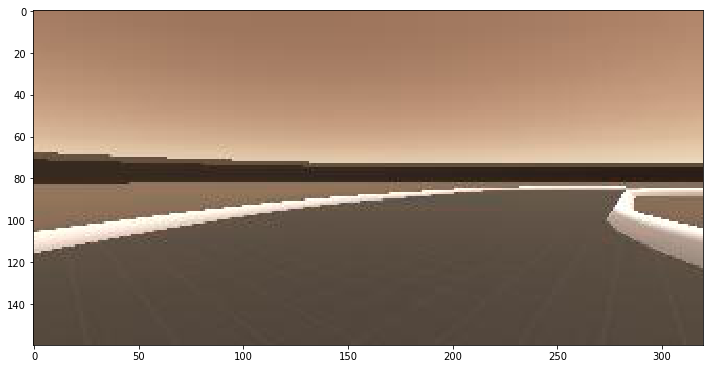
\includegraphics{img/sim_img.png}}
  }
  \caption{Obraz z symulatora}
  \label{sim_img}
\end{figure}
\begin{figure}
  \centering
  \fbox{
  \scalebox{0.5}{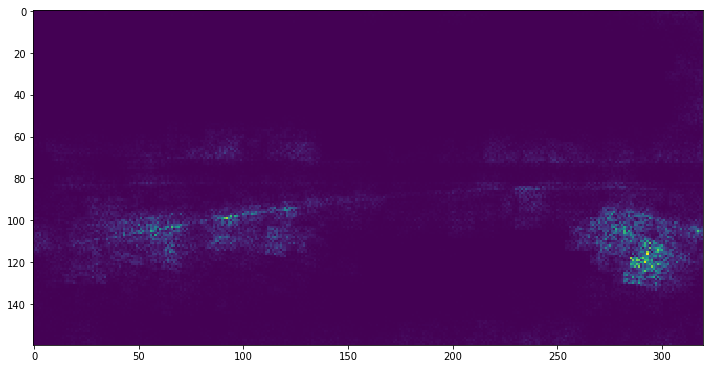
\includegraphics{img/sim_img_act.png}}
  }
  \caption{Na co sieć patrzy, symulator}
  \label{sim_act}
\end{figure}
\begin{figure}
  \centering
  \fbox{
  \scalebox{0.5}{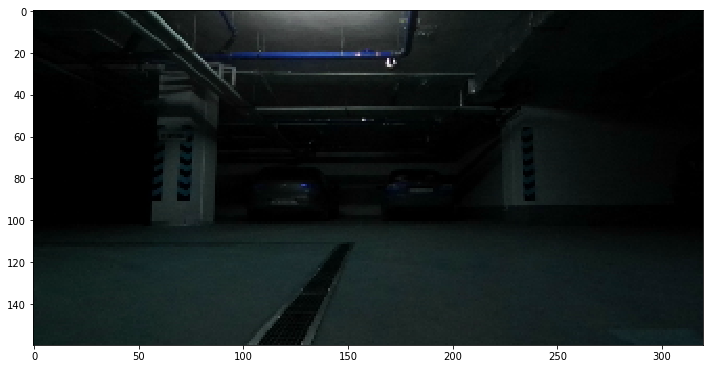
\includegraphics{img/real_img.png}}
  }
  \caption{Obraz z nagrania}
  \label{real_img}
\end{figure}
\begin{figure}
  \centering
  \fbox{
    \scalebox{0.5}{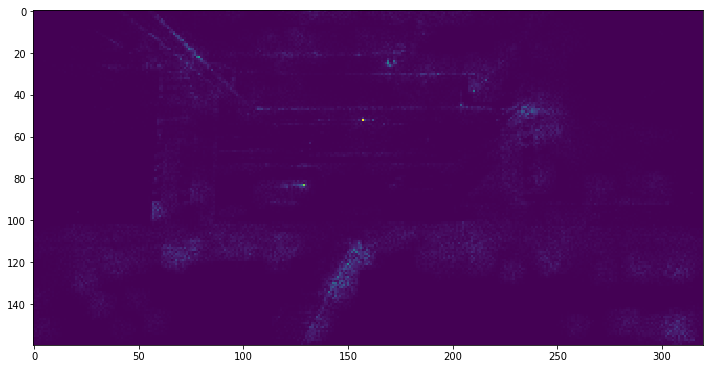
\includegraphics{img/real_img_act.png}}
  }
  \caption{Na co sieć patrzy, nagranie}
  \label{real_act}
\end{figure}

Z kolei dla łazika intensywność w najbardziej aktywnym miejscu jest dużo mniejsza \ref{real_act}.
Oznacza to, że nie sugeruje się tylko jednym obszarem z kamery. Najbardziej jednak 
zwraca uwagę na kratkę na podłodze, która mogłaby wystarczyć do nawigacji.

\section{W porównaniu do nagrania}
Na wykresie \ref{plot_ang} widać, że sieć (pomarańczowy kolor) mniej gwałtownie 
zmienia szybkość obrotu niż kierowca (kolor niebieski). Jednak sieć reaguje w podobnych momentach co kierowca na konieczność wykonania skrętu.

\begin{figure}
  \centering
  \fbox{
    \scalebox{0.5}{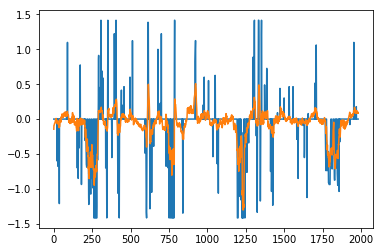
\includegraphics{img/real_data_ang.png}}
  }
  \caption{Prędkość obrotowa: sieć vs kierowca}
  \label{plot_ang}
\end{figure}

\section{Wpływ architektury}
W przypadku sieci pod symulator, usunięcie niektórych warstw konwolucyjnych
pozwalało modelowi nadal utrzymywać się na torze, natomiast taka sama zredukowana architektura 
nie radziła sobie dobrze w przypadku nagrań z prawdziwego łazika. Z kolei
usunięcie nieliniowości z warstw konwolucyjnych ograniczyło zdolności sieci do takiego stopnia,
że nie potrafiła się utrzymać na wirtualnym torze.

Usunięcie dropoutu bardzo szybko powodowało overfitting i sieć radziła sobie
dobrze tylko na danych uczących. Z kolei dodanie warstw liniowych na końcu nie 
poprawiało, ani nie pogorszało zbytnio wydajności sieci, przynajmniej dla
nagrań z symulatora. Na tej podstawie można wywnioskować, że większość interesujących 
cech obrazu została już znaleziona w ramach warstw konwolucyjnych, więc dla tak prostych danych zwiększenie modelu jest nieefektywne.

Co ciekawe, w przypadku wytrenowanego już modelu do symulatora zredukowanie 
rozdzielczości obrazów dziesięciokrotnie w każdym wymiarze (z rozdzielczości 
320x160 do 32x16),
i zwykłe przeskalowanie w górę przed zewaluowaniem wystarczy, żeby utrzymać się 
na torze.

Ponadto, sieć uczona na obrazie kolorowym działa bezproblemowo, gdy
zredukuje się obraz do skali szarości. Jedyne, co należy wykonać to stworzyć obraz kolorowy, w którym każdy z kanałów RGB będzie powtórzonym obrazem wejściowym.

